\documentclass[border=10pt]{standalone}
\usepackage{pgfplots}
\pgfplotsset{compat=1.18}
\begin{document}
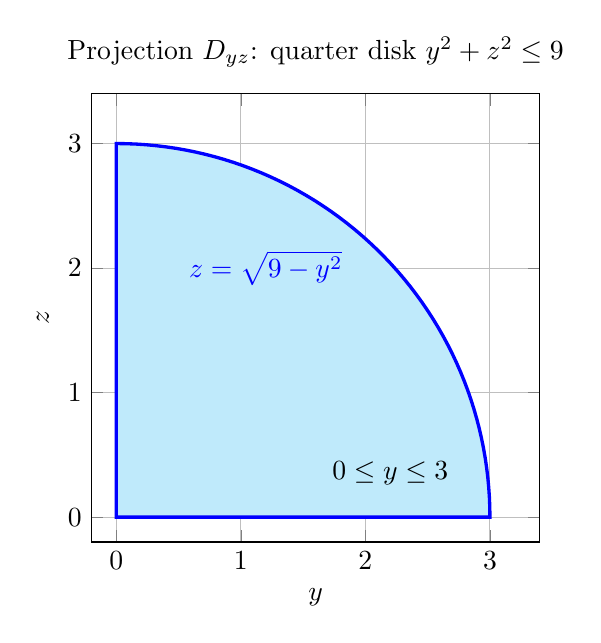
\begin{tikzpicture}
\begin{axis}[
    xlabel={$y$}, ylabel={$z$},
    xmin=-0.2, xmax=3.4, ymin=-0.2, ymax=3.4,
    grid=major, axis equal image,
    title={Projection $D_{yz}$: quarter disk $y^2+z^2\le 9$},
]
% Quarter disk
\addplot[fill=cyan!25, draw=blue, very thick, domain=0:90, samples=60]
    ({3*cos(x)}, {3*sin(x)}) \closedcycle;
% Label
\node[blue] at (axis cs:1.2,2.0) {$z=\sqrt{9-y^2}$};
\node at (axis cs:2.2,0.35) {$0\le y\le 3$};
\end{axis}
\end{tikzpicture}
\end{document}